\section{Adding a custom vehicle}
\label{sec:custom-vehicle}

To help reduce the gap between simulation and reality we created and imported a digital model of the NAPLab car to the CARLA simulator. In order to do this we first had to build CARLA from source to get access to the Unreal Editor, since this is not included in the packaged versions of the simulator. We followed CARLA's documentation\footnote{\url{https://carla.readthedocs.io/en/0.9.14/build_linux/}} to build CARLA from source on Ubuntu 20.04. Since this requires a computer with a display and an adequate GPU we used the new VCXR computer equipped with a NVIDIA RTX 4090 GPU.

Once the build process was done and we had access to the Unreal Editor, we could follow the guides on content authoring to start creating our custom vehicle. Note that there exist two guides describing this process which differ slightly in their instruction (\footnote{\url{https://carla.readthedocs.io/en/0.9.14/tuto_content_authoring_vehicles/}} and \footnote{\url{https://carla.readthedocs.io/en/0.9.14/tuto_A_add_vehicle/}}). Before doing any work in Unreal Editor however, we had to model our vehicle in Blender \cite{blender}.


\subsection{Modelling in Blender}

We were provided a 3D model (SDL file) of the Kia e-Niro that NAPLab uses from our supervisors. We imported this to Blender as seen in \cref{fig:blender-kia}.

\begin{figure}[h!]
    \centering
    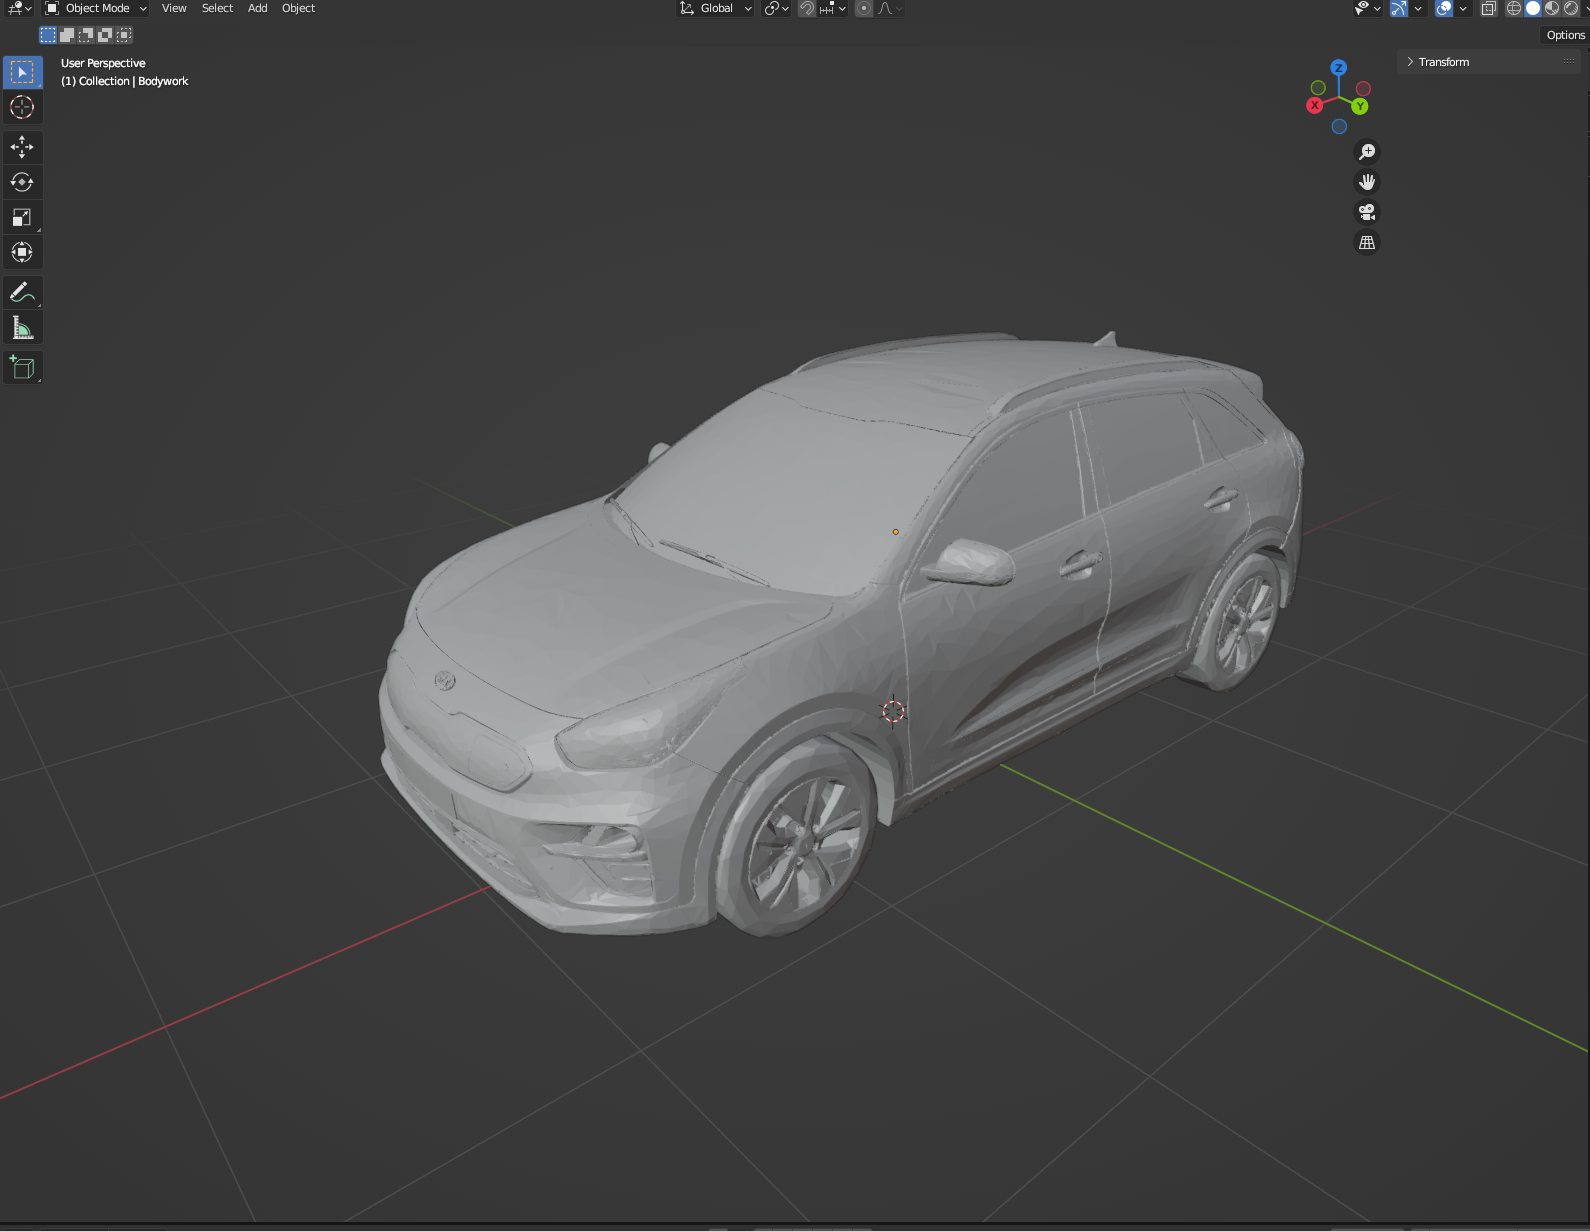
\includegraphics[width=.8\textwidth]{chapters/3-method/figures/blender-kia.png}
    \caption{Kia SDL file imported into Blender.}
    \label{fig:blender-kia}
\end{figure}

As recommended by CARLA we reduced the face count of the vehicle from over 1,000,000 down to around 100,000. This was done using Blender's decimate tool as seen in \cref{fig:blender-decimate}. 

\begin{figure}[h!]
    \centering
    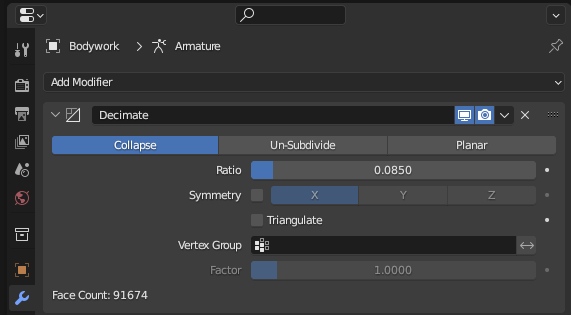
\includegraphics[width=.8\textwidth]{chapters/3-method/figures/blender-kia-decimate.png}
    \caption{The decimate settings used to reducuse the face count of the vehicle.}
    \label{fig:blender-decimate}
\end{figure}

CARLA requires that the wheels are separated from the main vehicle body. Our model consisted of one mesh, so we used Blender's tool for mesh selection and separation to create a standalone mesh for each wheel. When this was done we could move the wheels freely as seen in \cref{fig:blender-wheel}

\begin{figure}[h!]
    \centering
    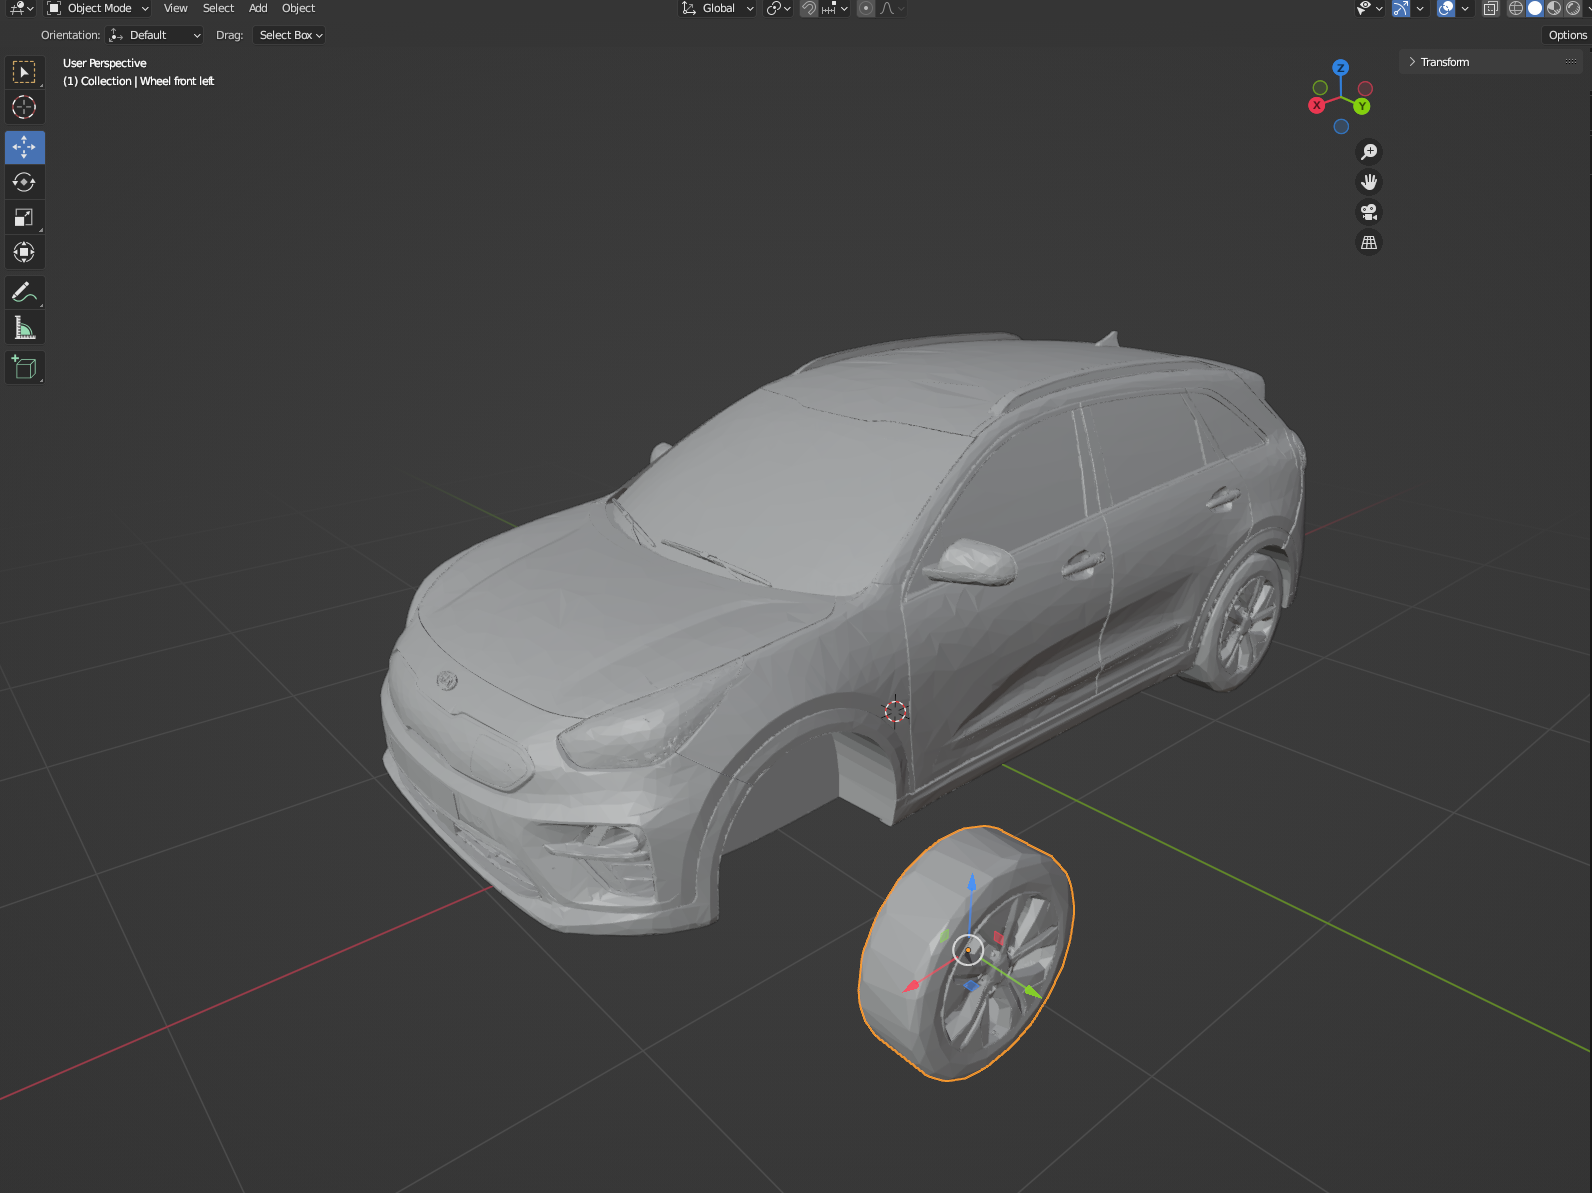
\includegraphics[width=.8\textwidth]{chapters/3-method/figures/blender-kia-wheel.png}
    \caption{The wheels could be moved independently after being separated from the main body.}
    \label{fig:blender-wheel}
\end{figure}

The last step in Blender was to rig an armature to our vehicle to identify the wheels and allow their movement. The armature consists of one main bone at the center of the vehicle and one connected bone per wheel, shown in \cref{fig:blender-armature}. The four wheel bones was placed in the center of each wheel, and allowed each wheel to rotate freely, while the main bone moves the whole vehicle.

\begin{figure}[h!]
    \centering
    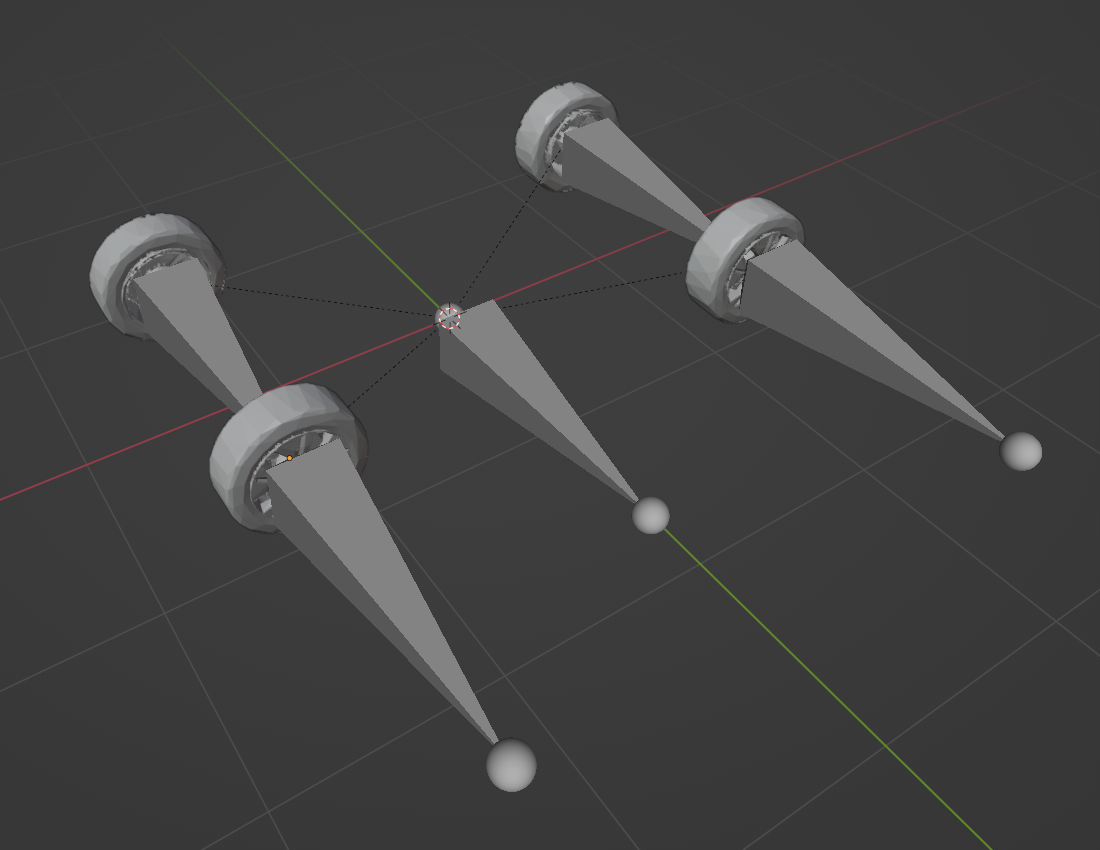
\includegraphics[width=0.7\textwidth]{chapters/3-method/figures/blender-kia-armature.png}
    \caption{The armature layout of the vehicle. There is one for each wheel and one for the vehicle as a whole.}
    \label{fig:blender-armature}
\end{figure}

The finished model was exported from Blender into FBX format for import into Unreal Editor.


\subsection{Importing into Unreal Editor}
We could now open the Unreal Editor. In \cref{fig:ue} we see a preview of the simulated world and the content browser at the bottom. 

\begin{figure}[h!]
    \centering
    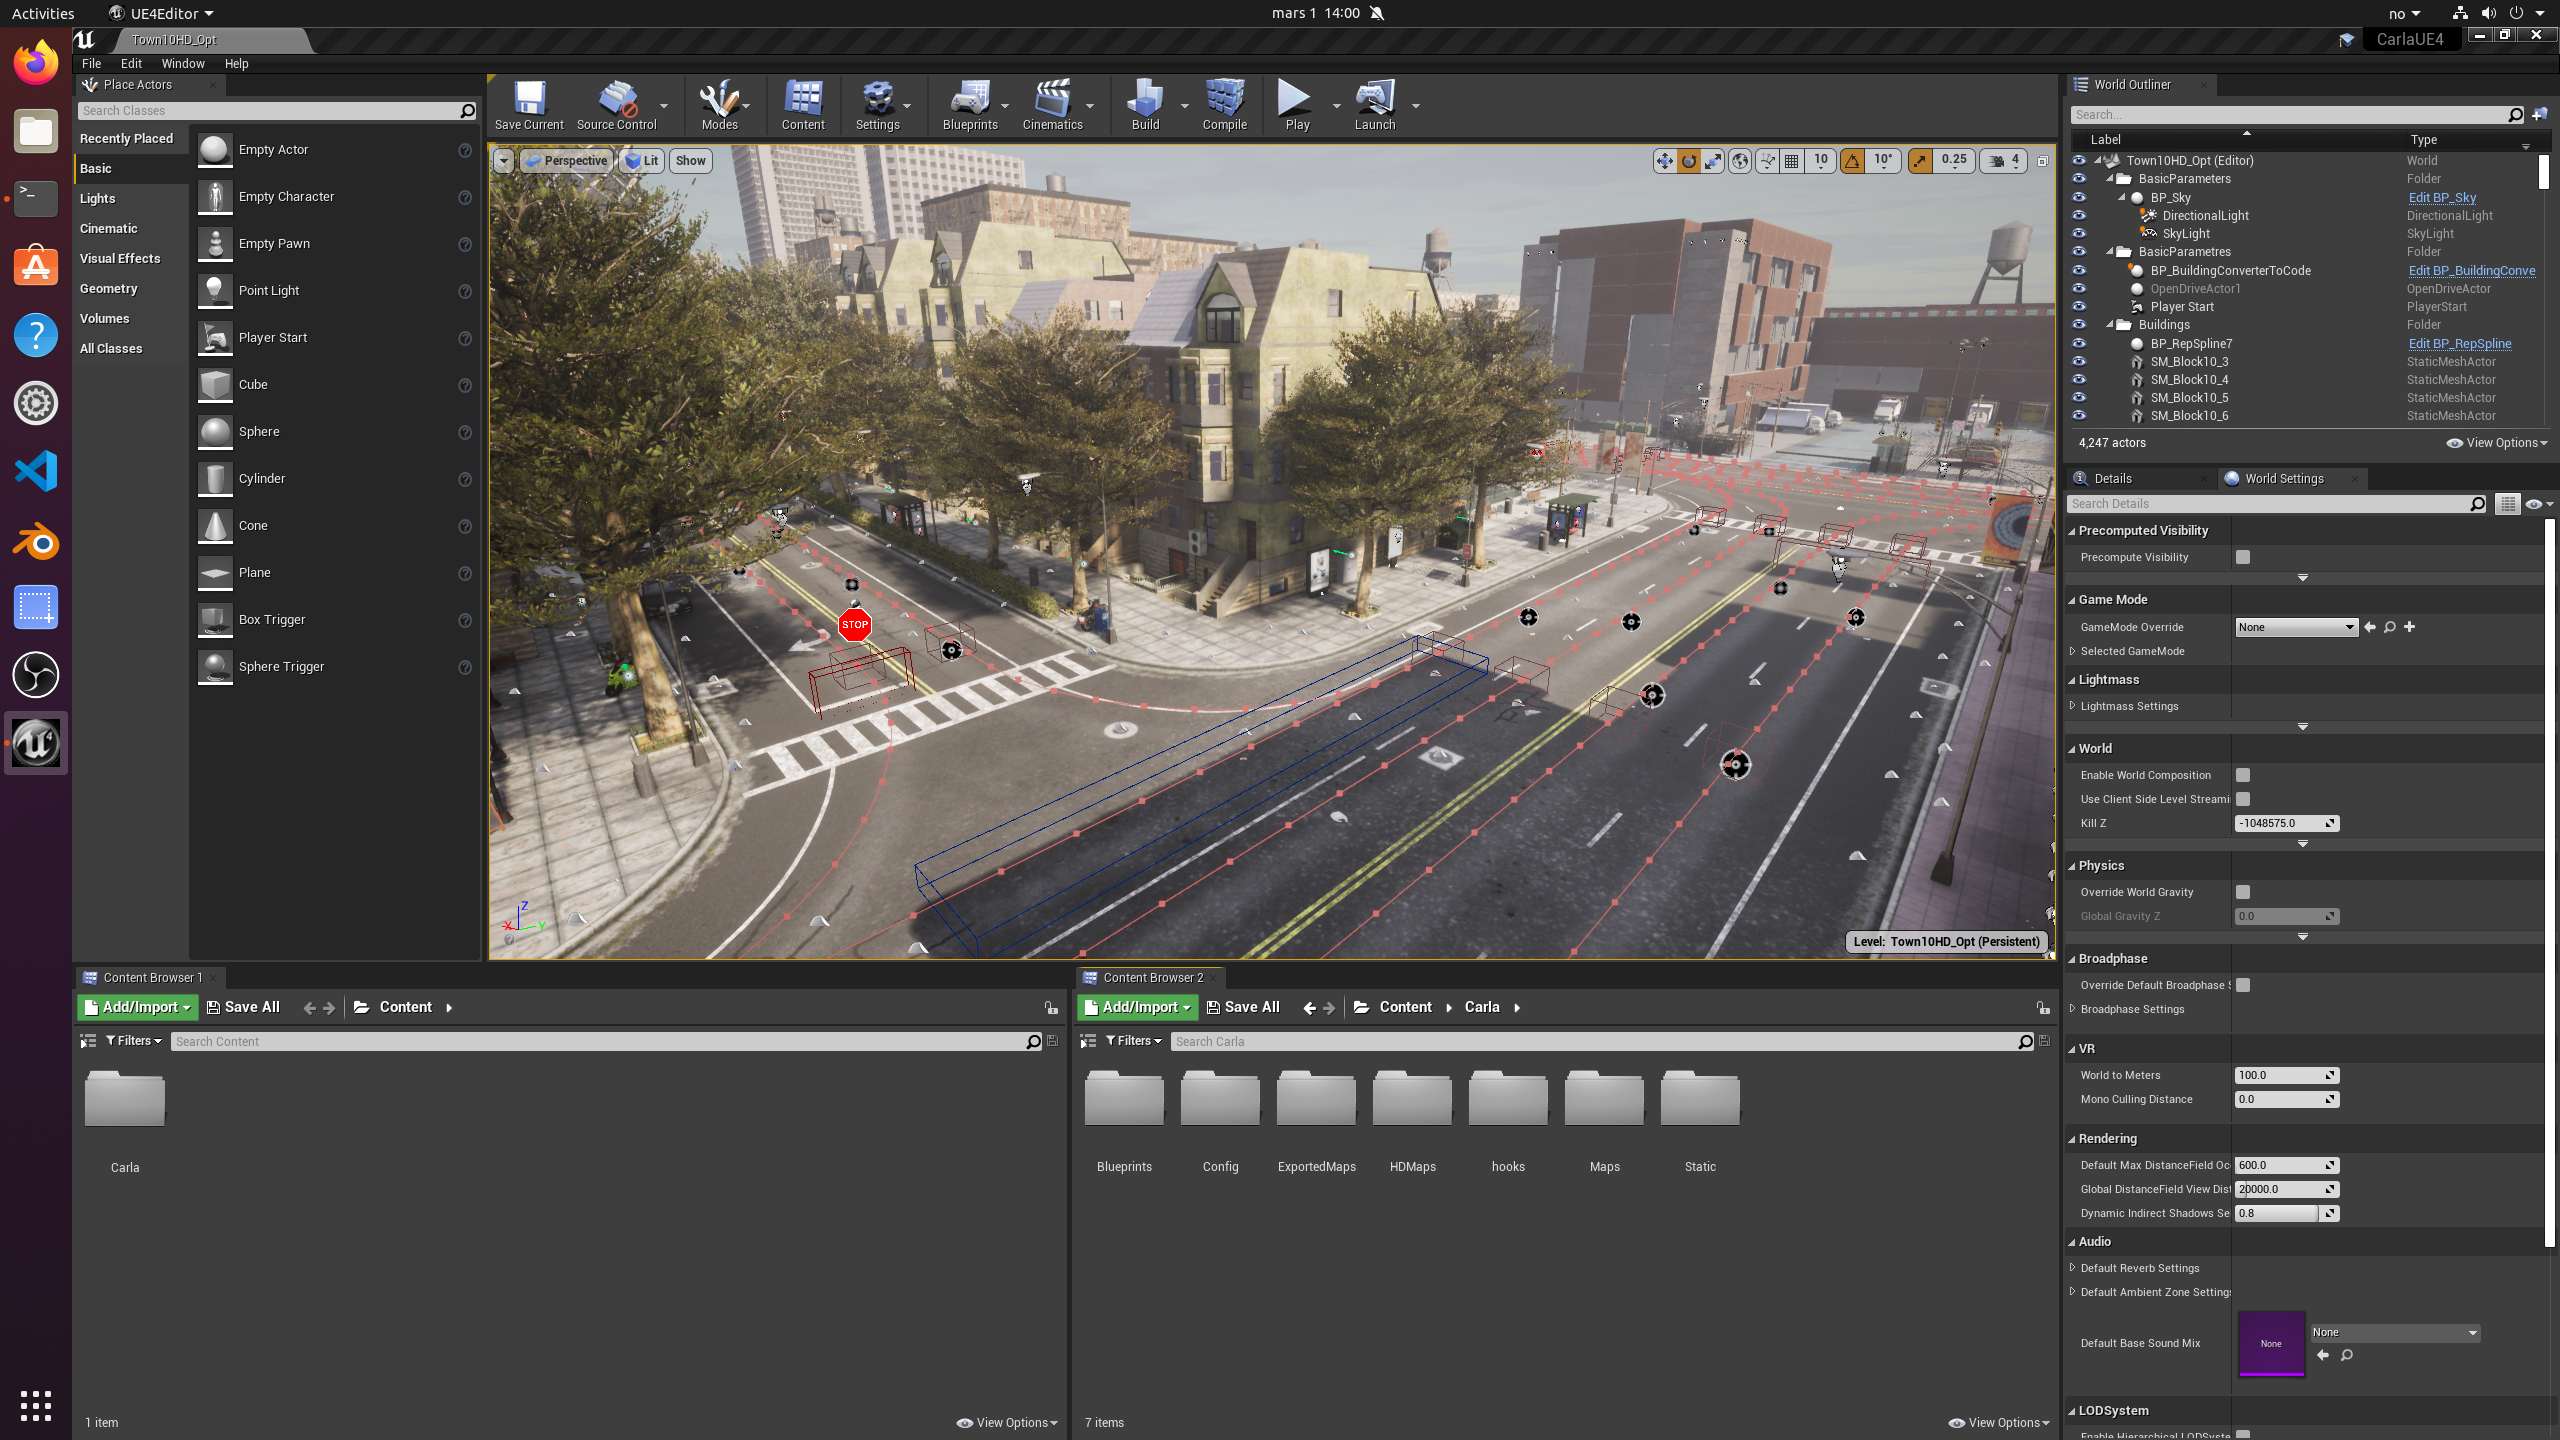
\includegraphics[width=\textwidth]{chapters/3-method/figures/ue.png}
    \caption{Custom version of Unreal Editor used for CARLA. The image showcases the simulator preview, content browser and properties panel.}
    \label{fig:ue}
\end{figure}

After importing the Kia FBX into Unreal Editor, we adjusted the physics asset to fit the car model as seen in \cref{fig:ue-kia-physics}. 

\begin{figure}[h!]
    \centering
    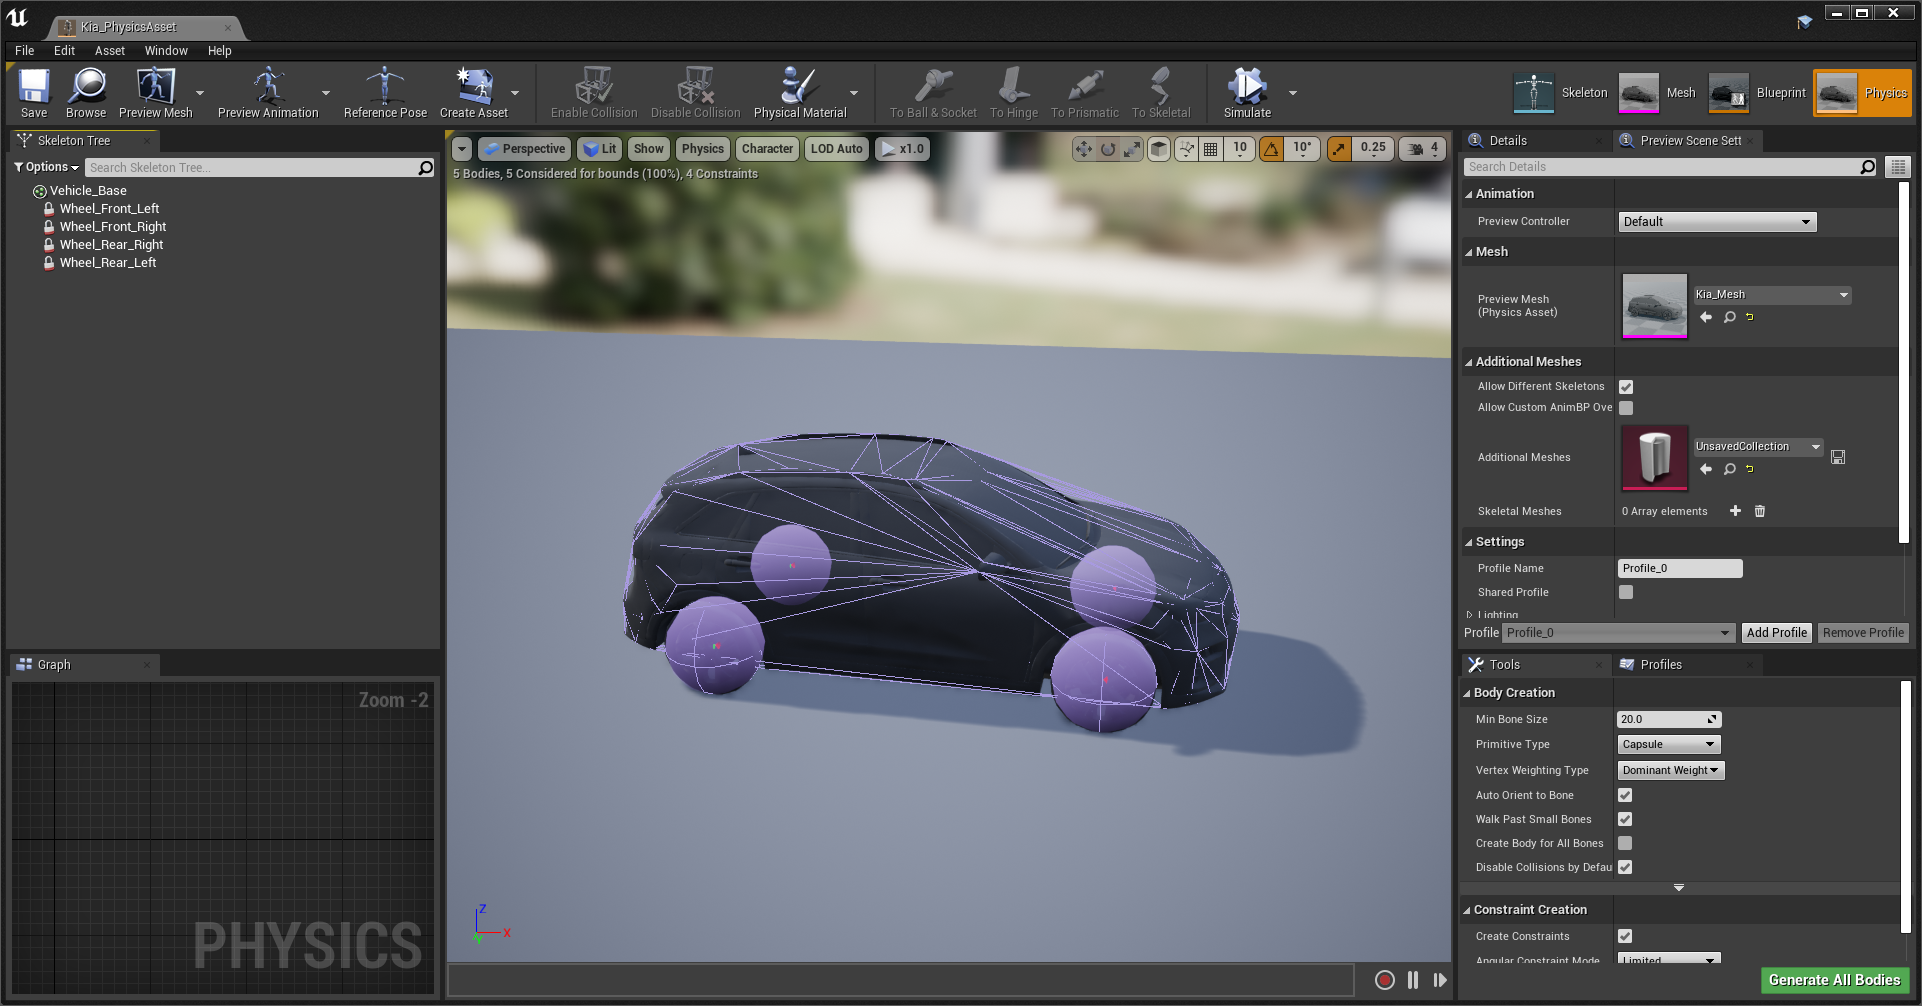
\includegraphics[width=\textwidth]{chapters/3-method/figures/ue-kia-physics.png}
    \caption{The Kia physics asset. It showcases the collision meshes for the wheels and main body.}
    \label{fig:ue-kia-physics}
\end{figure}

We then created an animation and blueprints for both the wheels and the car as a whole as specified by the documentation. To add lights to our vehicle we copied the front headlight objects from the Tesla Model 3 blueprint to our blueprint as seen in \cref{fig:adding-lights}. \cref{fig:comparing-lights-on-off} shows the effect of adding headlights. 

\begin{figure}[h!]
    \centering
    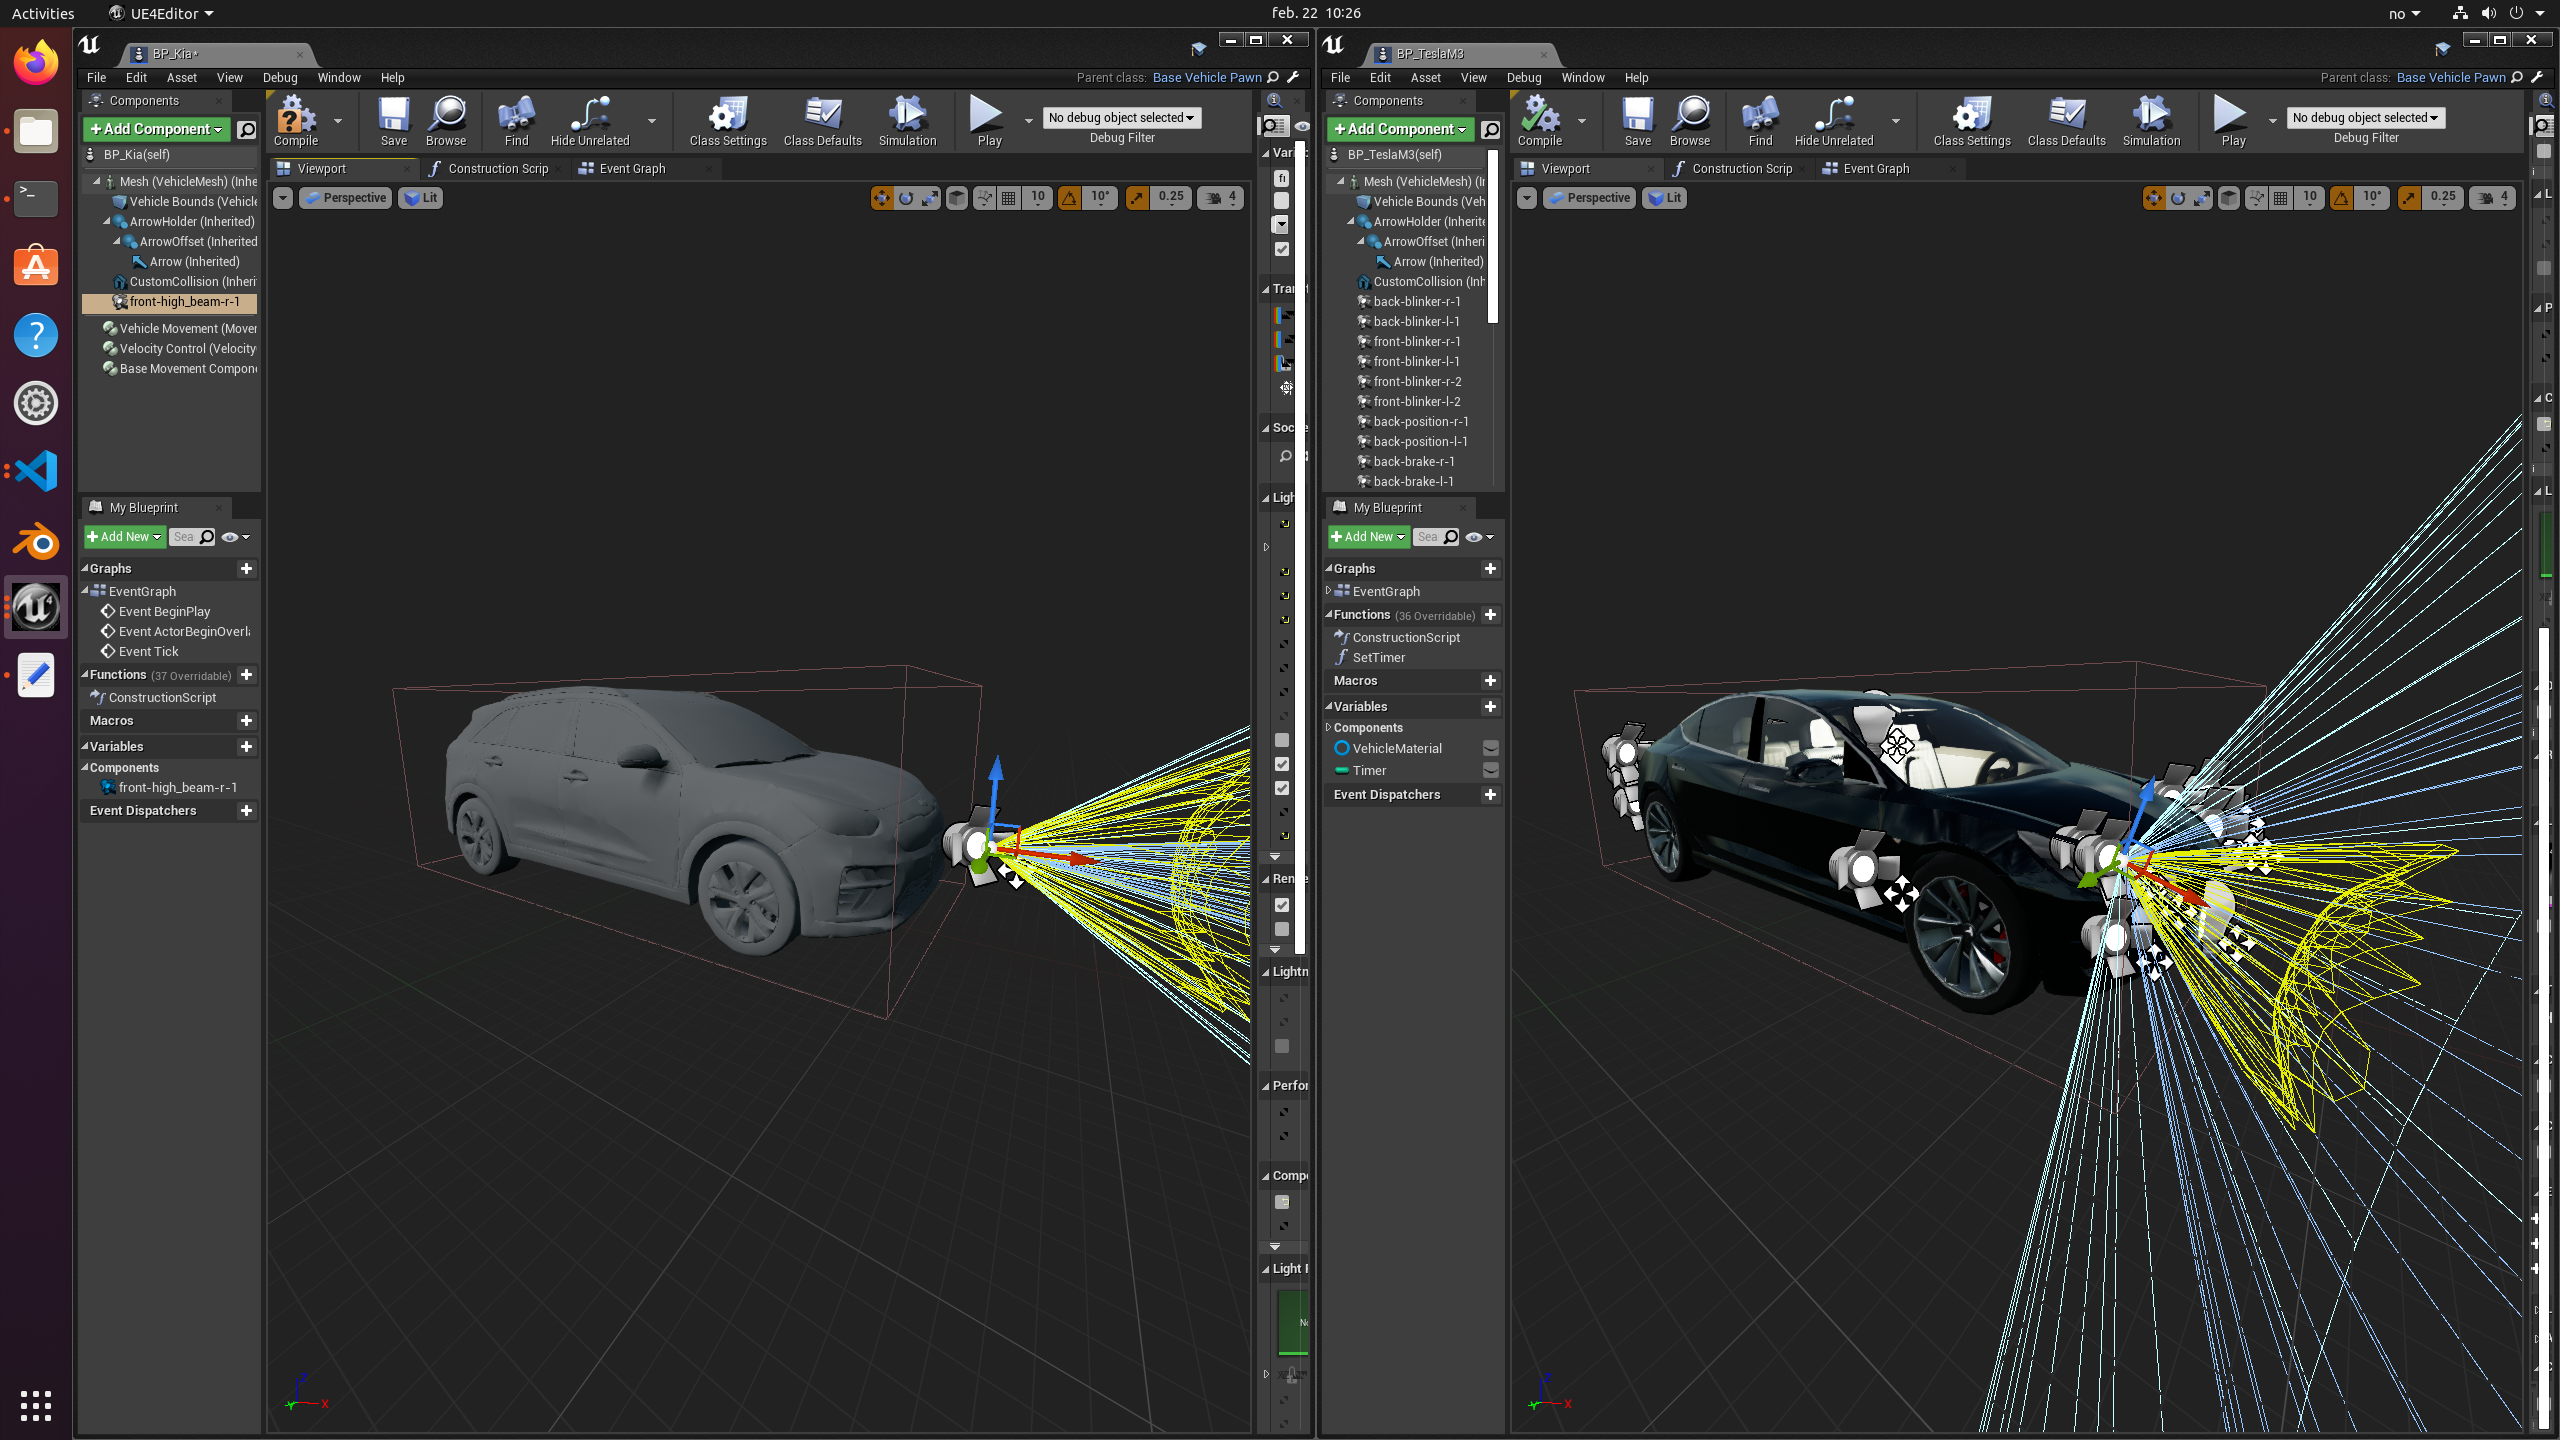
\includegraphics[width=\textwidth]{chapters/3-method/figures/adding-lights.png}
    \caption{To add lights to the new vehicle, we copied existing light objects from the Tesla Model 3 blueprint to the Kia blueprint.}
    \label{fig:adding-lights}
\end{figure}

\begin{figure}
    \centering
    \begin{subfigure}[h!]{0.49\textwidth}
        \centering
        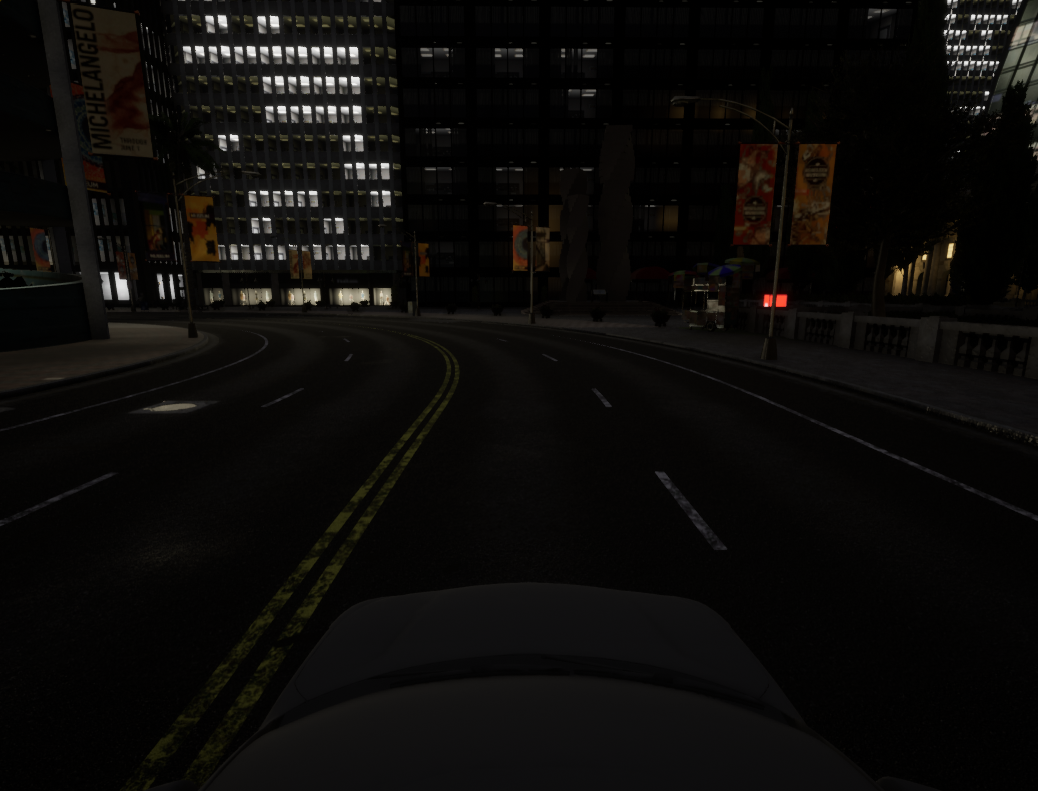
\includegraphics[width=\textwidth]{chapters/3-method/figures/lights-off.png}
        \caption{Lights off.}
        \label{fig:lights-off}
    \end{subfigure}
    \hfill
    \begin{subfigure}[h!]{0.49\textwidth}
        \centering
        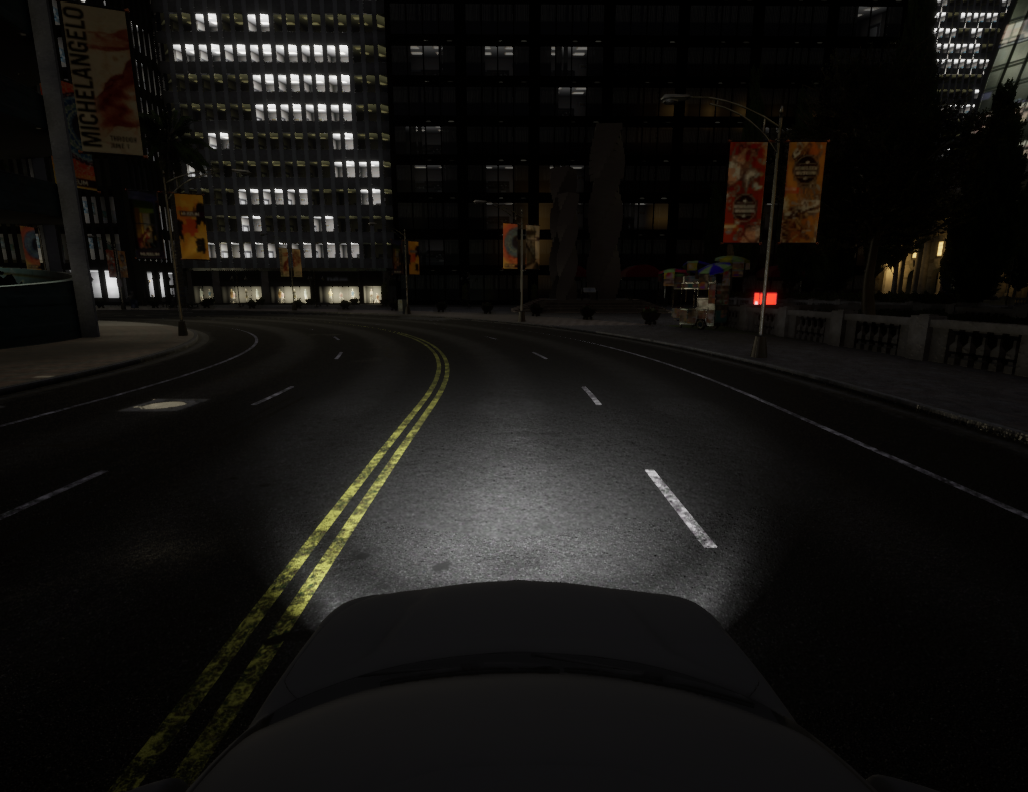
\includegraphics[width=\textwidth]{chapters/3-method/figures/lights-on.png}
        \caption{Lights on.}
        \label{fig:lights-on}
    \end{subfigure}
    \caption{Comparing before and after turning the vehicle lights on.}
    \label{fig:comparing-lights-on-off}
\end{figure}

The final list of assets is shown in \cref{fig:ue-kia-assets}. We can preview the vehicle in the simulator by dragging the car blueprint into the simulator window and pressing play as shown in \cref{fig:ue-kia}. Note that we also added a white car texture available in the simulator to the vehicle. This closely match the material of the real world car, and were good enough for our needs since we only see the vehicle from the perspective of the mounted cameras.

\begin{figure}[h!]
    \centering
    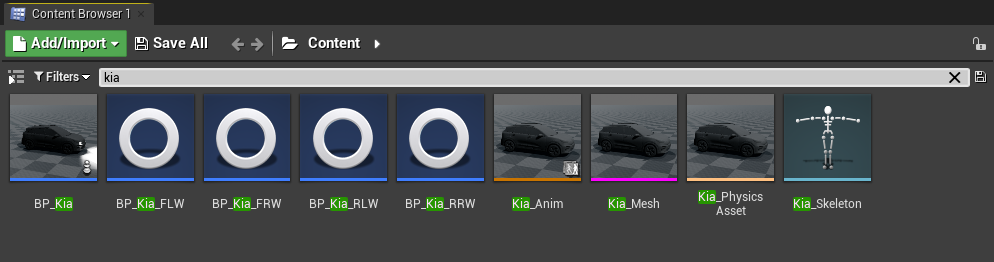
\includegraphics[width=\textwidth]{chapters/3-method/figures/ue-kia-assets.png}
    \caption{Final list of assets added for the new vehicle.}
    \label{fig:ue-kia-assets}
\end{figure}


\begin{figure}[h!]    
    \centering
    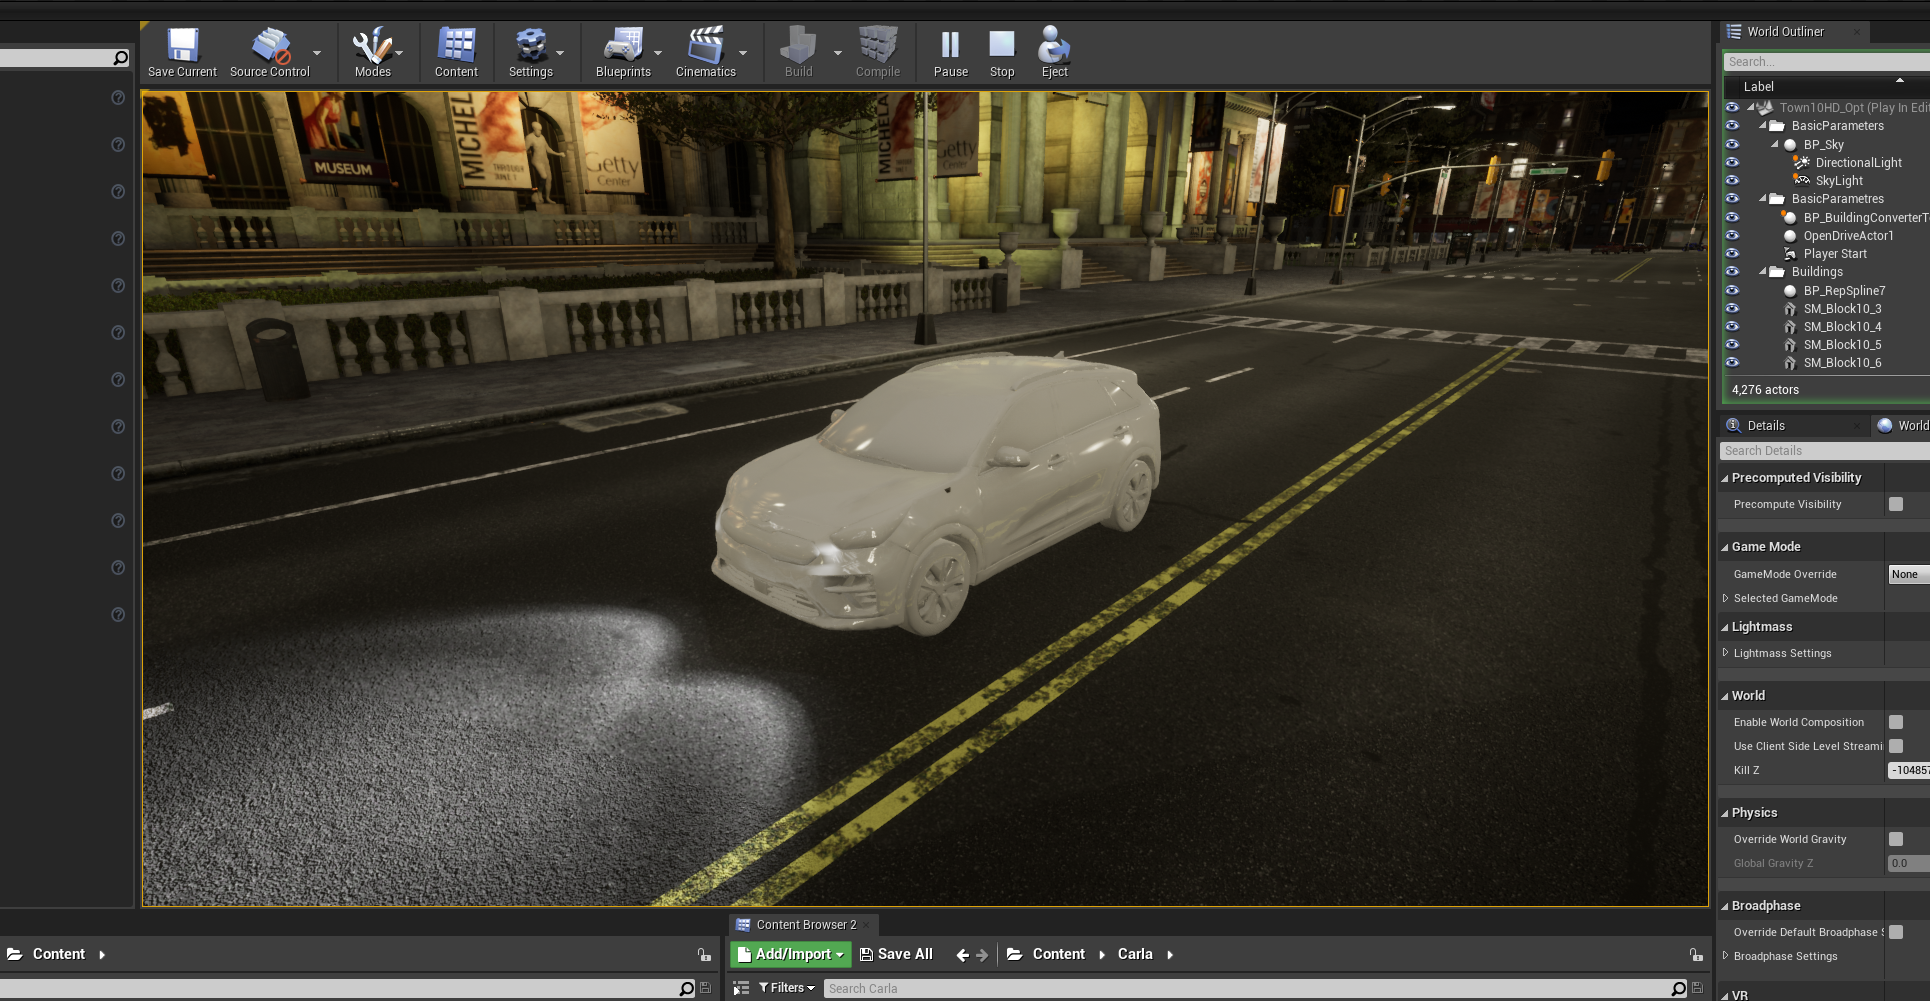
\includegraphics[width=\textwidth]{chapters/3-method/figures/ue-kia.png}
    \caption{Preview of the new vehicle in the simulator.}
    \label{fig:ue-kia}
\end{figure}


This concludes the process of adding our custom vehicle to the CARLA simulator. We have uploaded a custom CARLA docker image that contains the new car for others to use. It was packaged using the commands found in the CARLA documentation\footnote{\url{https://carla.readthedocs.io/en/0.9.14/tuto_A_create_standalone/}}. The docker image can be downloaded by running \texttt{docker pull mathiaswold/carla:0.9.14}, and the blueprint name is \texttt{'vehicle.kia.e-niro'}.
